\documentclass[11pt, oneside]{article}   	% use "amsart" instead of "article" for AMSLaTeX format
\usepackage{geometry}                		% See geometry.pdf to learn the layout options. There are lots.
\geometry{letterpaper}                   		% ... or a4paper or a5paper or ... 
%\geometry{landscape}                		% Activate for for rotated page geometry
%\usepackage[parfill]{parskip}    		% Activate to begin paragraphs with an empty line rather than an indent
\usepackage{graphicx}				% Use pdf, png, jpg, or eps� with pdflatex; use eps in DVI mode
								% TeX will automatically convert eps --> pdf in pdflatex		
\usepackage{amssymb}
\usepackage{amsmath}

\title{Differentiation Summary}
%\author{The Author}
%\section{}
% \subsection*{R code}
\date{}							% Activate to display a given date or no date

\graphicspath{{/Users/telliott_admin/Dropbox/Tex/png/}}

% \begin{center} 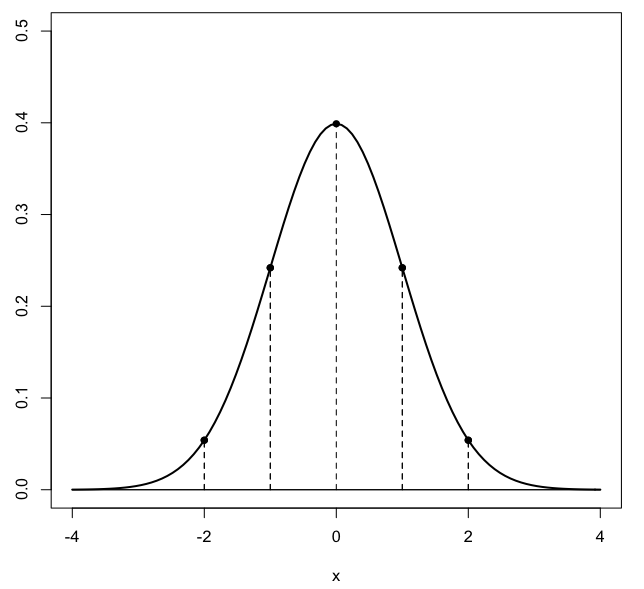
\includegraphics [scale=0.4] {gauss3.png} \end{center}
% \begin{bmatrix} a  &  b \\ c  &  d \end{bmatrix}
% \bigg |_

\begin{document}
\maketitle
\large
%\noindent
Here is a quick summary of what you will need to know (memorize) about basic differentiation.

\noindent
If $f(x) = ag(x)$ (with $a =$ constant) then
\[ f'(x) = ag'(x)  \]
If $f(x) = g(x) + h(x)$ then
\[ f'(x) = g'(x) + h'(x)  \]
\subsection*{power rule}
If $f(x) = x^n$ then
\[ f'(x) = nx^{n-1} \]
Together, these rules allow us to differentiate any polynomial function.

For the next part, it is convenient to use the symbols $y$ and $u$ when we mean $y(x)$ and $u(x)$ and $u'$ when we mean $u'(x)$
\subsection*{product and quotient rules}
If $y=uv$ then ("this times the derivative of that, etc...")
\[ y' = u'v + uv' \]
If $y=u/v$ then
\[ y' = \frac{u'v - uv'}{v^2} \]
With this last one, it can be hard to remember which term gets the minus sign.  Just check with $y = 1/x$
\[ y' = \frac{0 \times x - 1 \times 1}{x^2} = -\frac{1}{x^2} \]
which agrees with the result from the power rule.
\subsection*{chain rule}
We'll do this one with an example, and use the $dy$ notation.  Suppose $y = \sqrt{(1-x^2)}$.  Substitute $u = 1-x^2$  Then $y = \sqrt{u}$ and
\[ \frac{dy}{du} = \frac{1}{2}\frac{1}{\sqrt{u}} \]
Furthermore, since $u = 1-x^2$
\[ \frac{du}{dx} = -2x \]
We want $dy/dx$, but that is just
\[ \frac{dy}{dx} = \frac{dy}{du} \ \frac{du}{dx} = \frac{1}{2}\frac{1}{\sqrt{1-x^2}} (-2x) = -\frac{x}{\sqrt{1-x^2}} \]
\subsection*{implicit differentiation}
We'll do this one also with an example.  Consider a circle with radius $r$ and equation $x^2 + y^2 = r^2$.  Imagine that $x$ is a function of some other variable $t$ (perhaps, time).  Then $y$ is also a function of time.  Now take derivatives $d/dt$, by the chain rule
\[ \frac{d}{dt} y^2 = 2y \frac{dy}{dt} \]
\[ \frac{d}{dt} x^2 = 2x \frac{dx}{dt} \]
but since $r$ is a constant
\[ \frac{d}{dt} r^2 = 0 \]
Putting it together
\[ 2y\ \frac{dy}{dt} + 2x\ \frac{dx}{dt} = 0 \]
Now, \emph{multiply by $dt$}
\[ 2y dy + 2x dx = 0 \]
Rearrange to obtain
\[ \frac{dy}{dx} = -\frac{x}{y} \]


\subsection*{trigonometric functions}
If $f(x) = \sin  x$, then
\[ f'(x) = \cos  x \]
while if $f(x) = \cos  x$, then
\[ f'(x) = -\sin  x \]
As an exercise, you should try finding $f'(x)$ when $f(x) = \tan  x$ using these definitions and the quotient rule from above.
\subsection*{exponential}
Finally, if $f(x) = e^x$ then
\[ f'(x) = e^x \]
while if $f(x) = log(x)$---mathematicians usually write the \emph{natural} logarithm this way---then
\[ f'(x) = \frac{1}{x} \]



\end{document}  